%% ut-thesis.tex -- document template for graduate theses at UofT
%%
%% Copyright (c) 1998-2013 Francois Pitt <fpitt@cs.utoronto.ca>
%% last updated at 16:20 (EDT) on Wed 25 Sep 2013
%%
%% This work may be distributed and/or modified under the conditions of
%% the LaTeX Project Public License, either version 1.3c of this license
%% or (at your option) any later version.
%% The latest version of this license is in
%%     http://www.latex-project.org/lppl.txt
%% and version 1.3c or later is part of all distributions of LaTeX
%% version 2005/12/01 or later.
%%
%% This work has the LPPL maintenance status "maintained".
%%
%% The Current Maintainer of this work is
%% Francois Pitt <fpitt@cs.utoronto.ca>.
%%
%% This work consists of the files listed in the accompanying README.

%% SUMMARY OF FEATURES:
%%
%% All environments, commands, and options provided by the `ut-thesis'
%% class will be described below, at the point where they should appear
%% in the document.  See the file `ut-thesis.cls' for more details.
%%
%% To explicitly set the pagestyle of any blank page inserted with
%% \cleardoublepage, use one of \clearemptydoublepage,
%% \clearplaindoublepage, \clearthesisdoublepage, or
%% \clearstandarddoublepage (to use the style currently in effect).
%%
%% For single-spaced quotes or quotations, use the `longquote' and
%% `longquotation' environments.


%%%%%%%%%%%%         PREAMBLE         %%%%%%%%%%%%

%%  - Default settings format a final copy (single-sided, normal
%%    margins, one-and-a-half-spaced with single-spaced notes).
%%  - For a rough copy (double-sided, normal margins, double-spaced,
%%    with the word "DRAFT" printed at each corner of every page), use
%%    the `draft' option.
%%  - The default global line spacing can be changed with one of the
%%    options `singlespaced', `onehalfspaced', or `doublespaced'.
%%  - Footnotes and marginal notes are all single-spaced by default, but
%%    can be made to have the same spacing as the rest of the document
%%    by using the option `standardspacednotes'.
%%  - The size of the margins can be changed with one of the options:
%%     . `narrowmargins' (1 1/4" left, 3/4" others),
%%     . `normalmargins' (1 1/4" left, 1" others),
%%     . `widemargins' (1 1/4" all),
%%     . `extrawidemargins' (1 1/2" all).
%%  - The pagestyle of "cleared" pages (empty pages inserted in
%%    two-sided documents to put the next page on the right-hand side)
%%    can be set with one of the options `cleardoublepagestyleempty',
%%    `cleardoublepagestyleplain', or `cleardoublepagestylestandard'.
%%  - Any other standard option for the `report' document class can be
%%    used to override the default or draft settings (such as `10pt',
%%    `11pt', `12pt'), and standard LaTeX packages can be used to
%%    further customize the layout and/or formatting of the document.

%% *** Add any desired options. ***
\documentclass{ut-thesis}

%% *** Add \usepackage declarations here. ***
%% The standard packages `geometry' and `setspace' are already loaded by
%% `ut-thesis' -- see their documentation for details of the features
%% they provide.  In particular, you may use the \geometry command here
%% to adjust the margins if none of the ut-thesis options are suitable
%% (see the `geometry' package for details).  You may also use the
%% \setstretch command to set the line spacing to a value other than
%% single, one-and-a-half, or double spaced (see the `setspace' package
%% for details).

%%%%%%%%%%%%%%%%%%%%%%%%%%%%%%%%%%%%%%%%%%%%%%%%%%%%%%%%%%%%%%%%%%%%%%%%
%%                                                                    %%
%%                   ***   I M P O R T A N T   ***                    %%
%%                                                                    %%
%%  Fill in the following fields with the required information:       %%
%%   - \degree{...}       name of the degree obtained                 %%
%%   - \department{...}   name of the graduate department             %%
%%   - \gradyear{...}     year of graduation                          %%
%%   - \author{...}       name of the author                          %%
%%   - \title{...}        title of the thesis                         %%
%%%%%%%%%%%%%%%%%%%%%%%%%%%%%%%%%%%%%%%%%%%%%%%%%%%%%%%%%%%%%%%%%%%%%%%%

%% *** Change this example to appropriate values. ***
\degree{Master of Applied Science}
\department{Civil Engineering}
\gradyear{2019}
\author{Stepan Oskin}
\title{The design and implementation of the housing market database for Greater Toronto and Hamilton area.}

%% *** NOTE ***
%% Put here all other formatting commands that belong in the preamble.
%% In particular, you should put all of your \newcommand's,
%% \newenvironment's, \newtheorem's, etc. (in other words, all the
%% global definitions that you will need throughout your thesis) in a
%% separate file and use "\input{filename}" to input it here.


%% *** Adjust the following settings as desired. ***

%% List only down to subsections in the table of contents;
%% 0=chapter, 1=section, 2=subsection, 3=subsubsection, etc.
\setcounter{tocdepth}{2}

%% Make each page fill up the entire page.
\flushbottom


%%%%%%%%%%%%      MAIN  DOCUMENT      %%%%%%%%%%%%

\begin{document}

%% This sets the page style and numbering for preliminary sections.
\begin{preliminary}

%% This generates the title page from the information given above.
\maketitle

%% There should be NOTHING between the title page and abstract.
%% However, if your document is two-sided and you want the abstract
%% _not_ to appear on the back of the title page, then uncomment the
%% following line.
%\cleardoublepage

%% This generates the abstract page, with the line spacing adjusted
%% according to SGS guidelines.
\begin{abstract}
%% *** Put your Abstract here. ***
%% (At most 150 words for M.Sc. or 350 words for Ph.D.)

\end{abstract}

%% Anything placed between the abstract and table of contents will
%% appear on a separate page since the abstract ends with \newpage and
%% the table of contents starts with \clearpage.  Use \cleardoublepage
%% for anything that you want to appear on a right-hand page.

%% This generates a "dedication" section, if needed -- just a paragraph
%% formatted flush right (uncomment to have it appear in the document).
%\begin{dedication}
%% *** Put your Dedication here. ***
%\end{dedication}

%% The `dedication' and `acknowledgements' sections do not create new
%% pages so if you want the two sections to appear on separate pages,
%% uncomment the following line.
%\newpage  % separate pages for dedication and acknowledgements

%% Alternatively, if you leave both on the same page, it is probably a
%% good idea to add a bit of extra vertical space in between the two --
%% for example, as follows (adjust as desired).
%\vspace{.5in}  % vertical space between dedication and acknowledgements

%% This generates an "acknowledgements" section, if needed
%% (uncomment to have it appear in the document).
%\begin{acknowledgements}
%% *** Put your Acknowledgements here. ***
%\end{acknowledgements}

%% This generates the Table of Contents (on a separate page).
\tableofcontents

%% This generates the List of Tables (on a separate page), if needed
%% (uncomment to have it appear in the document).
%\listoftables

%% This generates the List of Figures (on a separate page), if needed
%% (uncomment to have it appear in the document).
%\listoffigures

%% You can add commands here to generate any other material that belongs
%% in the head matter (for example, List of Plates, Index of Symbols, or
%% List of Appendices).

%% End of the preliminary sections: reset page style and numbering.
\end{preliminary}


%%%%%%%%%%%%%%%%%%%%%%%%%%%%%%%%%%%%%%%%%%%%%%%%%%%%%%%%%%%%%%%%%%%%%%%%
%%  Put your Chapters here; the easiest way to do this is to keep     %%
%%  each chapter in a separate file and `\include' all the files.     %%
%%  Each chapter file should start with "\chapter{ChapterName}".      %%
%%  Note that using `\include' instead of `\input' will make each     %%
%%  chapter start on a new page, and allow you to format only parts   %%
%%  of your thesis at a time by using `\includeonly'.                 %%
%%%%%%%%%%%%%%%%%%%%%%%%%%%%%%%%%%%%%%%%%%%%%%%%%%%%%%%%%%%%%%%%%%%%%%%%

%% *** Include chapter files here. ***
\chapter[Background information]{Background information} \label{ch:background}

\section{Chapter 2: transportation and land use, land registration in Canada and Teranet} \label{sec:chapter_2_intro}

This chapter discusses the complex interaction of land use and transportation, provides a brief overview of the history of development of land use-transportation (LUT) models, presents some legal and historical background for Teranet's dataset of real estate transactions and finishes with discussing challenges of working with Teranet's data and the proposed solution.

\section{Land Use and Transport (LUT) models} \label{sec:evolution_of_models_of_urban_systems}

\subsection{Complexity of urban systems and "wicked" problems} \label{subsec:complexity_and_wicked_problems}

In her famous 1961 book, Jane Jacobs\cite{Jacobs1961} described a city as "a problem in organized complexity";
since then, many other researchers have remarked that urban systems exhibit complex behaviour\cite{Batty2008, Bettencourt2013}.
Complexity of a system can be defined as a state or quality of being intricate or complicated.
For a system to be complex is not necessarily the same as to be complicated;
complex systems can be simple, i.e.\ governed by a single equation.
Complexity of a system has to do with the intrinsic ability of a system to surprise us with its behaviour;
that the system is hard to understand, despite the mechanics of it being relatively simple.

In 1973, a little over a decade after Jacobs, Rittel and Webber\cite{Rittel1973} presented a path-breaking conceptualization;
this conceptualization characterized urban planning problems as "wicked" problems: problems which cannot be definitively described and for which it makes no sense to talk of "optimal solutions".
In their paper, Rittel and Webber stated that such "wicked" problems are never "solved", and that the focus instead becomes on iteratively "re-solving" the problems over and over.
More than 40 years after their original publication, Rittel and Webber's ideas remain relevant to the policy sciences today: there is an intense interest in the nature of "wicked" problems and the complex tasks of identifying their scope, viable responses, and appropriate mechanisms and pathways to improvement\cite{Crowley2017}.
Interaction between land use and transportation, which is discussed in the following section, presents a prime example of urban complexities and "wicked" problems.

\subsection{Transportation-land use cycle} \label{subsec:transportation_land_use_cycle}

Among the reasons why transportation and land use interaction is "wicked" are such aspects as pluralism of expectations among stakeholders, institutional complexity in policy making, and scientific uncertainty\cite{Noto2015}.
More importantly, there is a fundamental link between transportation and urban form: urban form has an enormous impact on the type and cost of transportation systems needed to serve residents of a metropolitan area\cite{Kelly1994}.
Transportation, in turn, influences land development and location choices of people and firms, and thus completes the formation of a feedback relationship that Stover and Koepke\cite{Stover1988} referred to as a cycle.
Interconnections between points (activities) in space can be perceived through the medium of the transportation system\cite{Miller1998}

Figure~\ref{fig:idealized_integrated_urban_model} illustrates the complex interactions between land use and transportation system as summarized by Miller, Kriger and Hunt\cite{Miller1998}.

\begin{figure}[hbt!]
    \centering
    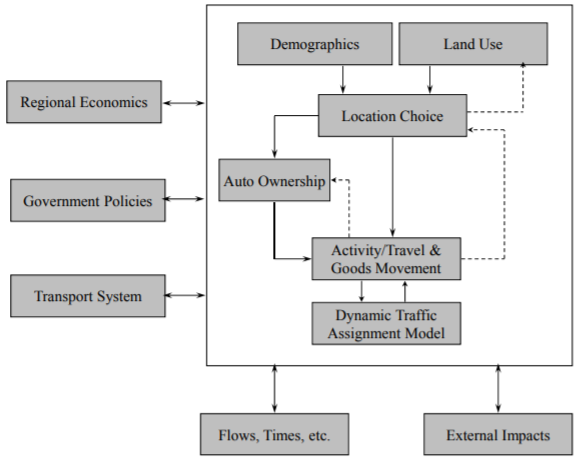
\includegraphics[width=0.7\linewidth,trim=0 0 0 0,clip]{miller_idealized_urban_model.png}
    \caption{An Idealized Integrated Urban Model System, adapted from Miller, Kriger and Hunt\cite{Miller1998}.}
    \label{fig:idealized_integrated_urban_model}
\end{figure}

Many different types of models are used in planning, such as demand forecasting models projecting traffic or ridership, or land use models projecting and distributing population and jobs within an area.
At an earlier stage of model development, some analysts argued that there is no significant link between transportation and land use, given the near-ubiquity of the transportation (road) network\cite{Miller1998}.
However, the unprecedented urban growth of the 21st century introduced new challenges for urban systems such as extreme road congestion, equity of access to jobs and services among low-income households, energy scarcity, environmental and GHG impacts from transportation systems and public health impacts of land use patterns\cite{Miller2018b,Moeckel2017}.

It became apparent that these "transport problems" cannot be solved through transportation policies and investment alone, that the physical design of the city at the "macro" and "micro" scale critically interfaces with the demand for and performance of the transportation system.
In addition, to accurately assess the costs and benefits of an expensive long-term transportation infrastructure investment, "feedback" effects of these investments on urban form, land values, property taxes, quality of life, etc.
need to be quantified and included in evaluation and decision making.
Thus, today there is a steadily growing recognition within the urban policy field that the interaction between transportation and land use does exist and does matter\cite{Miller2018b}.

%TODO change the end of 1st sentence
In the context of models, integrated urban models (IUMs) aim to capture the complex relationship between urban systems such as transportation and land use more accurately.
Integrated land use-transportation models combine travel demand forecasting and land use forecasting functions and recognize that the distribution of population and jobs depends, in part, on transportation accessibility.
The reverse is also true, and thus integrated models incorporate feedback relationship between transportation and land use, with economic decisions by households and firms acting as one of the links between the two systems\cite{Miller1998}.

\subsection{Evolution of LUT models} \label{subsec:evolution_of_lut_models}

The history of treating cities as systems via simulation models of transportation and land use dates back to 1950s when General System Theory and Cybernetics came to be applied in the softer social sciences\cite{Batty2008}.
The first operational simulation model that truly integrated land use and transportation is considered to be A Model of Metropolis built in 1964 by Ira S. Lowry for the Pittsburgh region based on economic base theory\cite{Lowry1964}.
It was a highly aggregate model based on theories of spatial interaction, such as the gravity model that was popular in quantitative geography and transportation planning at the time\cite{Bouchard1965}.
Models based on spatial interaction framework continued to be developed through mid-1980s, until developments in random utility theory allowed researchers to describe choices among discrete alternatives, such as the choice of travel mode, and generate models based on the study of disaggregate behaviour\cite{Iacono2008}.

Figure~\ref{fig:lut_model_evolution} provides the general overview of chronological development of LUT models summarized by Iacono\cite{Iacono2008}.

\begin{figure}[hbt!]
    \centering
    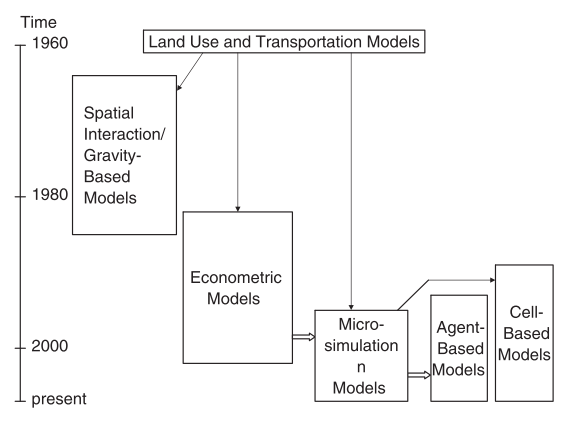
\includegraphics[width=0.7\linewidth,trim=0 0 0 0,clip]{lut_models_evolution.png}
    \caption{Chronological development of LUT models summarized by Iacono\cite{Iacono2008}.}
    \label{fig:lut_model_evolution}
\end{figure}

The modeling paradigm has changed fundamentally in the early 1990s along with the advances in computing power and efficiency of data storage.
Urban systems used to be viewed as hierarchical and centrally organized equilibrium structures, or "top-down".
Instead, now they were considered to be structured from the "bottom-up", dynamically retaining their integrity through interactions of numerous microelements\cite{Batty2008}.
A new broad class of LUT models that could fall under the title of "microsimulation" began to be developed.
It included such classes of models as activity-based travel, cell-based models, and multi-agent models, and more recently comprehensive urban microsimulation models that fully reflect the dynamics of changes in the population and the urban environment\cite{Iacono2008}.
%TODO check last sentence

"Micro" in the microsimulation implies that the model must be highly disaggregated spatially, socio-economically and in its representation of processes.
"Simulation" implies that the model must be numerical, stochastic, have an explicit time dimension, and "evolve" into the end state rather than "solve for it"\cite{Miller2018c}.
An example of such model has been developed by the University of Toronto ILUTE team;
their product is an integrated urban model capable of microsimulating urban demographic evolution, housing markets and travel behaviour over extended periods of time\cite{Miller2018a}.
The ILUTE system and some of the ways for its future improvement are discussed in the following section.

\subsection{ILUTE and HoMES model systems} \label{subsec:ilute}

The Integrated Land Use, Transportation, Environment (ILUTE) model system is an agent-based microsimulation model for greater Toronto-Hamilton area;
it includes such components as land use, activity/travel, urban economics, auto ownership, demographics and emissions/energy use.
It uses disaggregate models of spatial socioeconomic processes to evolve the state of the greater Toronto\textendash Hamilton area from a known base case to a predicted end state in 1-year time steps.
The system state is defined in terms of the individual persons, households, dwelling units, firms, etc.
that collectively define the urban region being modeled\cite{Miller2011}.

ILUTE model simulates the evolution of an urban region's spatial form, demographics, travel behavior and economic structure over time.
Many markets are of interest within ILUTE, such as housing, labour, commercial, real estate, etc.) and are modeled via microsimulation.
The model aims to capture the dynamics of these markets through disaggregated representations.
For example, in the housing market component of ILUTE, houses are auctioned off one dwelling at a time to interested bidders in a disaggregate implementation of Martinez' Bid Choice theory\cite{Martinez1992}.

The Housing Market Evolutionary System (HoMES) is the updated housing market module for the ILUTE model system.
HoMES is a disaggregate, agent-based microsimulation of the owner-occupied housing market that evolves the residential location of households over time and includes the endogenous supply of housing by type and location, as well as the endogenous determination of sales prices and rents.

An overview of the framework of housing market supply, demand and clearing mechanisms utilized in HoMES provided by Rosenfield et al.\cite{Rosenfield2013} is presented on figure~\ref{fig:homes_framework}

\begin{figure}[hbt!]
    \centering
    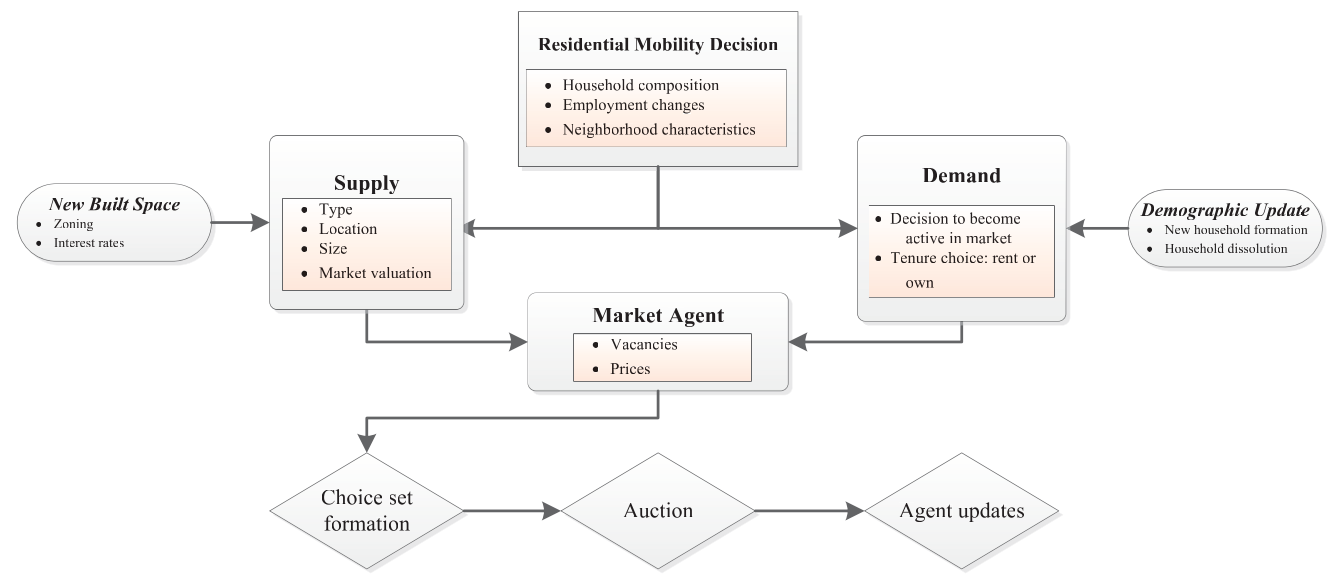
\includegraphics[width=0.99\linewidth,trim=0 0 0 0,clip]{homes_framework.png}
    \caption{Framework of housing market supply, demand and clearing mechanisms used in HoMES module of ILUTE, as summarized by Rosenfield et al.\cite{Rosenfield2013}.}
    \label{fig:homes_framework}
\end{figure}

Among the major barriers to implementation of integrated urban models since their introduction were such aspects as data hungriness and computational requirements\cite{Miller1998}.
However, continuing methodological advances, such as cost-effective High Performance Computing (HPC), detailed GIS-based datasets and machine learning methods, mean that former barriers now represent opportunities for model system development.
In the case of ILUTE and HoMES, one of the possibilities for further improvement is the use of new data sources to update the housing market model.
One of these new data sources, Teranet's dataset of land registry records, and main challenges of working with it are discussed in section~\ref{sec:new_data_sources_and_their_challgenges}.

\section{New data sources and their challenges} \label{sec:new_data_sources_and_their_challgenges}

\subsection{Further improvement of integrated urban models} \label{subsec:further_improvement_of_iums}


As an increasing amount of aspects of human life becomes digitalized, a wealth of new data is produced and can be used to model and analyze dynamics of urban systems\cite{Arribas-Bel2014, Chen2016}.
An example of such digitalization of human activity is the introduction of the Province of Ontario Land Registration Information System (POLARIS) in 1985 by the Government of Ontario\cite{TeranetEnterprisesInc.} that will be discussed in the following section.
Introduction of POLARIS lead to the creation of an extensive dataset of real estate transactions (land registration records) by the Teranet Enterprises Inc.
This dataset offers a very fine resolution of housing market dynamics across both time and space, which can be beneficial for updating and testing microsimulation models, but it also presents challenges to work with that will be discussed in section~\ref{subsec:teranet_ontario} of this chapter;
the chapter concludes with the proposed solution to address one of the main challenges of working with Teranet's data.

\subsection{POLARIS: electronic system of land registration in Ontario} \label{subsec:land_reg_system_canada}

All land owned in Canada is registered in a public land registry in the applicable province.
Each province and territory in Canada has its own land registry system, whether it is a land titles system, a registry system or a combination of both, with each system having its own rules.
The registry system is a public record of documents evidencing transactions affecting land.
In the land titles system, the applicable provincial government determines the quality of the title, and essentially guarantees (within certain statutory limits) the title to, and interests in, the property.
As of 2015, most common law provinces and territories in Canada were using the land titles system or were in the process of converting from a registry system to a land titles system\cite{McKean2015}.

As of 2015, the Province of Ontario has largely converted from registry systems to a land titles system.
In 1985, the Government of Ontario initiated the Province of Ontario Land Registration Information System (POLARIS) pilot project for the purposes of the conversion between systems and records automation.
The Land Registration Reform Act (Ontario)\cite{TheGovernmentofOntario1990} was introduced in 1990 to facilitate electronic search and registration of properties and the automation of paper-based records.
POLARIS was built by the Province to house and process electronic land records, which in turn lead to the creation of an extensive dataset of land registration records managed by Teranet Enterprises Inc.
Today, POLARIS is the search/registration and property maintenance system for all automated land records in Ontario.

\subsection{The Teranet-Ontario Partnership, Teranet's data and its challenges} \label{subsec:teranet_ontario}

In 1991, the Government of Ontario established a partnership with Teranet, a Toronto-based organization, founded the same year, which provides e-services to legal, real estate, government, financial, and healthcare markets.
The partnership was established to convert Ontario's land registration system to a more modernized electronic title system.
The project involved taking a 200-year-old paper-based system and creating a database with electronic records for more than five million parcels of land.
Teranet converted all qualified Registry properties in Ontario to the Land Titles system and automated existing paper Land Titles parcels.
As a result, 99.9\% of property in Ontario was parcelized and administered under the Land Titles system.
Teranet fully automated the conversion of millions of paper-based documents and records into the Ontario Electronic Land Registration System (ELRS)\cite{TeranetEnterprisesInc.2019}.


Teranet dataset presents an extensive historical record of real estate transactions recorded in the Province of Ontario since the beginning of XIX century.
However, when it comes to using new data sources in social studies, along with opportunities there are also challenges present.
For example, these data sources can have issues with the quality of the data, might require a specific set of skills to take advantage of these data sources, or might not be suitable for traditional methods meant for traditional data\cite{Arribas-Bel2014}, all of which are true in the case of Teranet's dataset.

One of the major attributes missing from the available version of Teranet's dataset is the information about the type of property being transacted, with records of various residential, commercial and industrial properties all being mixed together in the same dataset.
At the same time, Teranet records have timestamps (dates) and location information (x and y coordinates) and thus can be joined to variety of other urban data sources, such as Census demographics, Transportation Tomorrow Survey (TTS) and parcel-level land use information.
It is possible to derive this attribute from additional related sources of information, such as detailed land use or Census demographics.
However, joining these data sources together requires additional considerations, as they use different spatial units and are available at different temporal spans, as will be discussed in chapter~\ref{ch:spatial_and_temporal_relationships_between_urban_data}.


\section{Chapter summary} \label{sec:background_summary}

The fundamental link between transportation and urban form creates a feedback relationship between land development, travel needs, viability of alternative modes, accessibility, and other important characteristics of the urban transportation system.
Numerous "top-down" and "bottom-up" models have been designed to analyze and forecast the behaviour of urban regions and interaction of their transportation and land use systems.
Since urban systems are complex in nature and require "re-solving" over and over, data science process models present a good fit for this task with their iterative structure.

Increased digitization of human activity, such as introduction of POLARIS land registration system by the Government of Ontario in 1985, produce a wealth of new information that can be used to study interaction between land use and transportation at a fine spatial and temporal scale.
Teranet's dataset of real estate transactions presents a wealth of information on the housing market of Ontario and can be used for empirical studies of transportation-land use interaction.
However, along with the opportunities, the new data sources also present new challenges.
Teranet's dataset has some data quality issues that need to be addressed and might require special skills to work with due to its size.
But most importantly, it is very limited in the number of features available for each transaction.

One of the major attributes missing from the available version of Teranet's dataset is the information about the type of property being transacted, with records of various residential, commercial and industrial properties all being mixed together in the same dataset.
At the same time, Teranet records have timestamps (dates) and location information (x and y coordinates) and thus can be joined to variety of other urban data sources, such as Census demographics, Transportation Tomorrow Survey (TTS) and parcel-level land use information.
It is possible to derive this attribute from additional related sources of information, such as detailed land use or Census demographics.
However, joining these data sources together requires additional considerations, as they use different spatial units and are available at different temporal spans, as will be discussed in chapter~\ref{ch:spatial_and_temporal_relationships_between_urban_data}.



%% This adds a line for the Bibliography in the Table of Contents.
\addcontentsline{toc}{chapter}{Bibliography}
%% *** Set the bibliography style. ***
%% (change according to your preference/requirements)
\bibliographystyle{plain}
%% *** Set the bibliography file. ***
%% ("thesis.bib" by default; change as needed)
\bibliography{thesis}

%% *** NOTE ***
%% If you don't use bibliography files, comment out the previous line
%% and use \begin{thebibliography}...\end{thebibliography}.  (In that
%% case, you should probably put the bibliography in a separate file and
%% `\include' or `\input' it here).

\end{document}
